\section{Predicting the signed displacement before fitting the instruments}
We tested whether the leading matrices in Theorems~2 and~3 predict individual fits at finite spacings. The test used a fresh set of initial conditions, independent of every earlier block. For each equation we drew eight blocks of 32 trajectories. We constructed POD bases from the current states at 37 anchor times $0.05,0.075,\ldots,0.95$, giving 1,184 rows per fit. We used ranks 6 and 10, one and two lags, and seven spacings from $0.00025$ to $0.025$. One arm held the response horizon at $0.005$. The other used the next state at horizon $h$.

At each anchor the semidiscrete right-hand side $f(u)$ and its Jacobian action $f'(u)f(u)$ supplied the first two time derivatives. Each was projected through the fixed POD basis. For a quadratic feature $q_iq_j$ we used $(q_iq_j)''=q_i''q_j+2q_i'q_j'+q_iq_j''$. Neither derivative was estimated from the lagged design. We integrated both semidiscrete equations with fourth-order exponential time differencing, using the original spatial grids and a time step of $0.000125$. A second integration halved the step for block zero of each equation.

\paragraph{Prediction and scoring.}
For each block we stored the signed leading matrices and angular constants, then recorded a SHA-256 digest of the prediction archive before running the scoring stage. The fixed-horizon prediction used the current OLS residual. The coupled prediction used only the current state and its derivatives. To score them, we fit the projected regression on the lagged observations. We computed the difference both by directly fitting state increments and by applying the residual identity in \eqref{eq:shift}. Working in the orthonormal coordinates of $U$ preserves the Frobenius norm and inner product of the fitted changes.

For prediction $\widehat D$ and measured displacement $D$, we scored magnitude and direction jointly with $e=\|\widehat D-D\|_{\F}/\|D\|_{\F}$ and separately recorded the Frobenius cosine. A zero prediction gives $e=1$. Before simulation we defined a usable prediction by $e\le0.25$ and cosine $\ge0.95$, subject to full numerical rank and a displacement above $10^{-13}\|Y-q(0)\|_{\F}$. For each equation, rank, lag count and response arm, the usable range extends from the smallest spacing through the last consecutive grid point with at least seven of eight blocks passing at every point. This definition describes the tested grid. It does not interpolate a continuous cutoff or treat spacings within one block as independent.

\begin{table}[ht]\centering\small
\caption{Maximum spacing in the prespecified usable range. Each entry requires at least seven of eight passing blocks throughout the grid prefix. The final columns give median observed powers $\log_2(\|D(2h)\|/\|D(h)\|)$ at the two smallest spacings with coupled horizon.}\label{tab:ranges}
\begin{tabular}{lrrrrrrr}\toprule
 & & \multicolumn{2}{c}{Fixed horizon} & \multicolumn{2}{c}{Coupled horizon} & \multicolumn{2}{c}{Power}\\
Equation &$r$ & 1 lag & 2 lags & 1 lag & 2 lags & 1 lag & 2 lags\\\midrule
\tableinput ranges.tex
\bottomrule\end{tabular}
\end{table}

At the smallest spacing the predicted coupled displacement had a median relative error below one percent for both lag counts. Its magnitude scaled approximately as $h^2$ and $h^4$, respectively (Table~\ref{tab:ranges}). At the largest spacing the two-lag prediction often missed the tolerance. The fixed-horizon two-lag prediction deteriorated sooner in both equations. With $h=\tau=0.005$ the theoretical one-quarter magnitude ratio predicts a relative error near $0.75$ for the sequential approximation. The fixed-horizon PDE formula uses the measured residual at the chosen horizon. It retains higher powers of the horizon in its coefficient, whereas the separable Lorenz--96 comparator below uses the first Taylor term of that coefficient. The median error of the fixed-horizon PDE formula was $\SequentialError$ and its median cosine was $\SequentialCosine$. On the very same data, the median predicted-to-measured magnitude ratio rose from $\SequentialRatio$ under Theorem~2 to $\CoupledRatio$ under Theorem~3. The median absolute relative error of the angular factor was $\AngleError\%$. Thus the missing response term accounts for a magnitude discrepancy that a check of the angle alone would miss. This comparison motivated the external test of \eqref{eq:cross} below.

\begin{figure}[ht]\centering
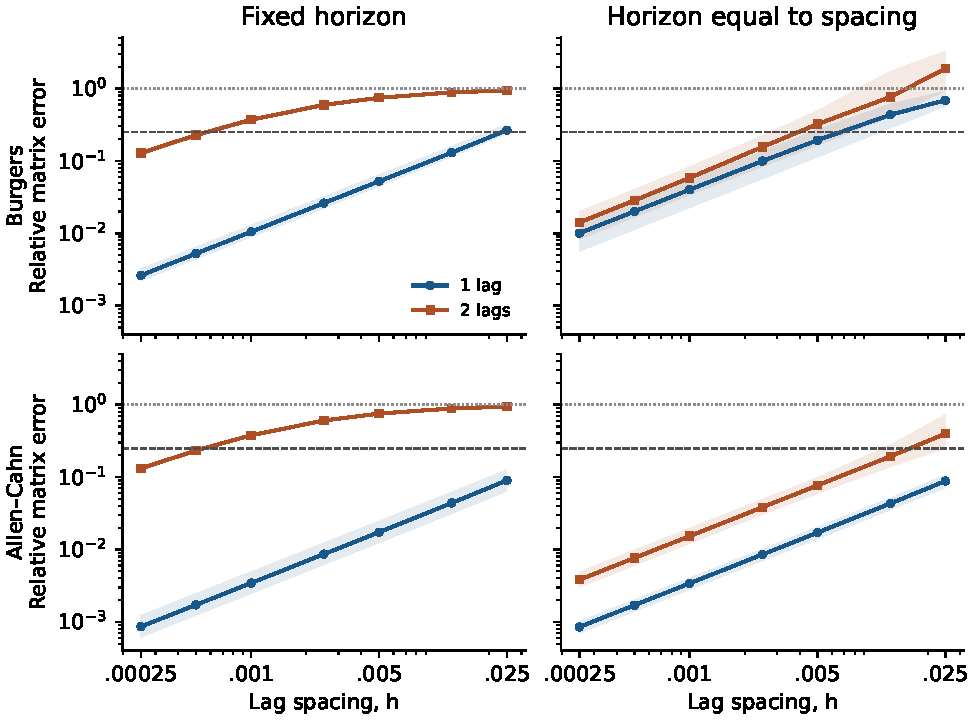
\includegraphics[width=.91\linewidth]{prediction.pdf}
\caption{Prospective relative matrix errors at rank 10. Curves give medians and bands span all eight independent blocks. The dashed line marks the error tolerance of 0.25. The dotted line at one gives the error of predicting zero.}\label{fig:prediction}
\end{figure}

All 896 primary evaluations and 112 integration checks had full numerical rank and resolved displacement. The maximum relative discrepancy between the direct and residualized fit differences was $\DirectDiff$, at a displacement of order $10^{-12}$. Halving the integration step changed the fitted displacement on the common spatial grid by approximately $\RefineDiff$ at its maximum in relative norm across the repeated blocks. The comparison assesses temporal resolution at the specified spatial grid.

\paragraph{A snapshot-only implementation.}
The equation derivatives provide a controlled check. In offline identification, one can instead observe the state at intermediate times. As a separate sensitivity analysis on the same blocks, we acquired three clean forward snapshots per anchor at offsets $\delta,2\delta,3\delta$, with $\delta=0.00075$. These auxiliary times are disjoint from every anchor, lag and response time used for scoring. Writing $d_j=q(j\delta)-q(0)$, we estimated $q'$ by $(18d_1-9d_2+2d_3)/(6\delta)$ and $q''$ by $(-5d_1+4d_2-d_3)/\delta^2$. We used these derivatives in the same formulas with the frozen basis and thresholds. The estimator needs only the four measured states for each derivative calculation. The simulator supplied those additional samples.

Across the 896 predictions the auxiliary-snapshot and equation-based calculations agreed on the pass/fail decision in \SnapshotAgreement{} cases. They gave identical usable grid prefixes in \SnapshotSame{} of the 16 equation, rank, lag-count and horizon combinations. The auxiliary measurements are clean and more frequent than the original training snapshots. Second differentiation scales observation errors by $\delta^{-2}$, so this check does not establish the accuracy of numerical derivatives in the noisy setting of Table~\ref{tab:noise}.
